\documentclass{article}
\usepackage[utf8]{inputenc}
\usepackage{amsmath}
\usepackage{listings}

\usepackage{amsthm}
\usepackage{graphicx}
\usepackage{upgreek}
\usepackage{algorithm}
\usepackage{algpseudocode}


\date{04 February 2019}
\marginparwidth 0.5in 
\oddsidemargin 0.25in 
\evensidemargin 0.25in 
\marginparsep 0.25in
\topmargin 0.25in 
\textwidth 6in \textheight 8 in
\newtheorem{question}{Question: }
\theoremstyle{case}
\newtheorem{case}{Case}
\graphicspath{ {images/} }
\begin{document}
\author{Sai Vineet Reddy Thatiparthi}

 \title{%
  Advanced Machine Learning \\
  \large Homework 2}
\maketitle
\textbf{The program is attached along with the submission. One has the option of training the program or loading the .h5 file of the already trained model to run computations and predictions on. Code written in Python3.}
\begin{enumerate}
    \item [A.] \textbf{Reserve about 20 percent of the data from each of the 62 classes for testing. Use the training data to construct a CNN that achieves as good a performance on the test data as possible. You can use
your favorite framework though you must be able to demonstrate
the running of your program}
\end{enumerate} 
\begin{proof} 
The code is attached.
\end{proof}

\begin{enumerate}
    \item [B.] \textbf{Display the confusion matrix (rows are actual classes, columns
are predicted classes). An entry is 1 if the truth agrees with the
prediction. Display the confusion matrix as an image. Comment
on the confusion matrix you obtained.}
\end{enumerate}
\begin{proof}
The confusion matrix can be seen in the Figure 1. The confusion matrix that I obtained seems to show that my CNN has predicted with a high degree of accuracy. However, one can see that this accuracy is sort of bi-modal, ie the prediction accuracy is higher with upper case letters (lower class numbers), but this accuracy goes down as the estimator wrongly predicts that lower case letters (higher class numbers) as upper case letters as seen in the confusion matrix.\\ \\ But despite this, one can clearly see the diagonal on the confusion matrix indicating mostly correct predictions. 
\begin{figure}[h]
            \caption{Confusion Matrix}
            \centering
            \includegraphics[scale=0.8]{img1.png}
            
            \end{figure}

\end{proof}
\begin{enumerate}
    \item [C.] \textbf{Focus on the first convolution layer. Examine the feature maps
and comment on what they evolved to detect. Be specific and cast
your answer in terms of the task i.e. what of the characters are
they detecting}
\end{enumerate} 
\begin{proof} 
\begin{figure}[t]
\centering
            \caption{Number 8}
            \includegraphics[scale=0.7]{img5.png}
            
            \end{figure}
\begin{figure}[t]
\centering
            \caption{What the first layer detects}
            \includegraphics[scale=0.6]{img4.jpg}
            
            \end{figure}
    
            \begin{itemize}
\item The image of number '8' was fed into the model and the outputs are displayed in the figures below. Look at Figure 3.
\item It is clear from the images below that some of the feature maps of the first convolution layers are detecting the edges of the character while others are detecting the inside edges of the feature maps. They have evolved to almost sketch their own copy of the character being passed in.

\item Basically, these feature maps have evolved to look for the major and main features of the image supplied. This isolates the primitive and basic features of the image. It looks for the simplest features that are common with all images, for example - a feature map that looks for curves in the number 8.
\item The feature maps of the first layer evolve to to activate when a specific feature is found. One can see that the output of this convolution layer is human readable.
\end{itemize}
\end{proof}

\begin{enumerate}
    \item [D.] \textbf{Focus on your last convolution layer. Examine the feature maps and
comment on what they evolved to detect. Be specific and cast
your answer in terms of the task i.e. what of the characters are
they detecting and in terms of what the earlier convolution layers
detected.}
\end{enumerate} 
\begin{proof}
\begin{figure}[t]
\centering
            \caption{What the last layer detects}
            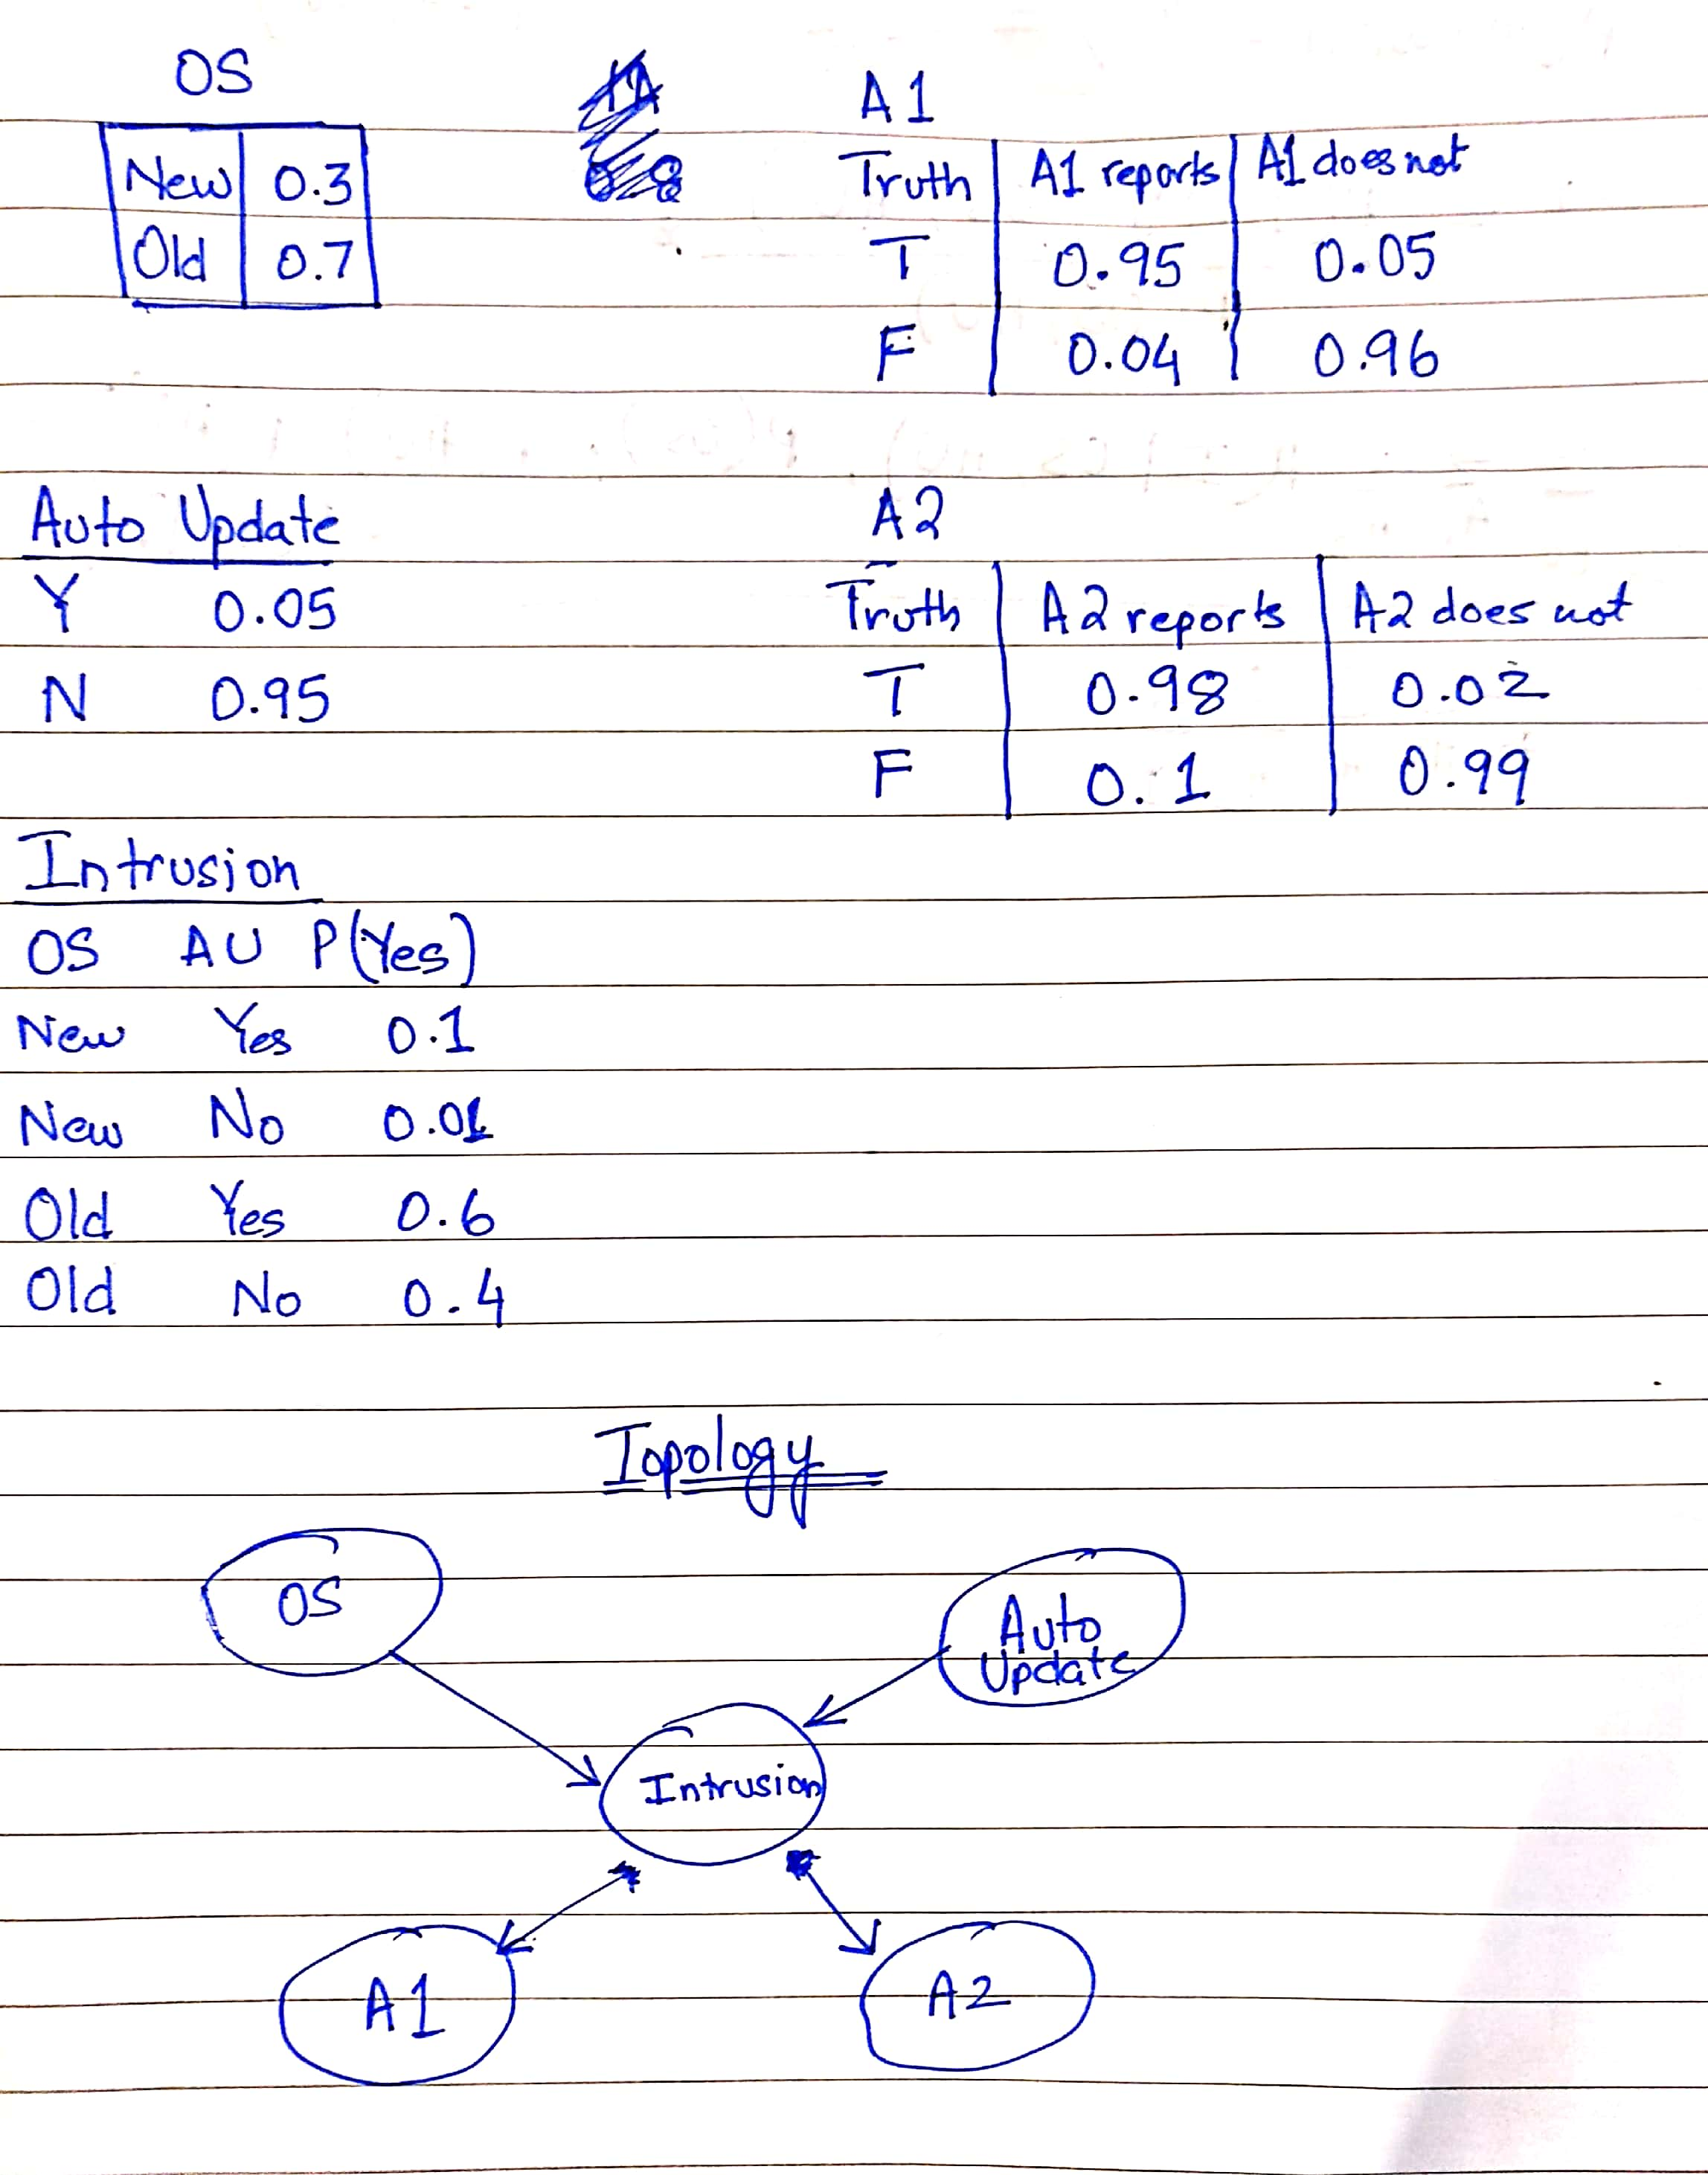
\includegraphics[scale=0.6]{img3.jpg}
            
            \end{figure}
            \begin{itemize}
                \item We will still be talking about the same number 8 being supplied to the model. Look at Figure 4.
                \item The last convolution layer receives, as its input, other, the output of every other convolution layer. This means that while its predecessors evolved to detect simple features such as lines and curves, our last layer evolved to detect and activate when it finds more and more complex features.
                \item This is achieved by combining what the earlier layers do (detect primitive features), and activating when a certain combination of features is passed down as input to the last layer. These feature combinations are usually not human understandable.
                \item An interesting thing is that this last layer gets a lot more information in the same receptive field (larger area of the input image considered in one go) than the earlier layers due to information compression caused about by the maxpool layers.
            \end{itemize}
. 
\end{proof}
\begin{enumerate}
    \item [E.] \textbf{What does stride control in a CNN. When would you use a larger/smaller
stride? Be specific.}
\end{enumerate} 
\begin{proof} 
Stride is the hyperparameter that decides how a feature map convolves around an image. This means that it controls how many pixels at once does a certain filter shift by each time it has to traverse over any given image. When the stride is one, we move the filter by 1 pixel, and when the stride is 2, we move the filter by 2 pixels each time. \\ \\
\textbf{Smaller stride - }
\begin{itemize}
    \item When a model needs to work with images that have a lot of important detail within them, using a small stride makes more sense.
    \item This is because, a small stride moves the feature map only by a bit each time, preserving the detail to great degree.
    \item This, however, increases the number of parameters as the feature map has to worry about more pixels because it moves very little each time. 
\end{itemize}

\textbf{Larger stride - }
\begin{itemize}
    \item When a model needs to work with images that do not have a lot of detail in them, one can choose to go with a large stride.
    \item This is because, a large stride moves the feature map by a large amount each time. This increases the information loss but since the image is not very detailed, it does not matter to us that the information is being lost.
    \item Since the feature map convolves a lot lesser with a large stride, the number of parameters decreases by a large degree as the feature map focuses (and repeats) on fewer pixels.  
\end{itemize}

\end{proof}
\end{document}